\documentclass[12pt,a4paper]{article}

% ─── Page Layout ───────────────────────────────────────────────────────────────
\usepackage[a4paper, margin=0.8in, headheight=14pt]{geometry}

% ─── Fonts (XeLaTeX) ───────────────────────────────────────────────────────────
\usepackage{fontspec}
\usepackage{unicode-math}
\setmainfont{TeX Gyre Pagella}
\setmonofont[Scale=0.88]{TeX Gyre Cursor}
\setmathfont{Latin Modern Math}

% ─── Packages ──────────────────────────────────────────────────────────────────
\usepackage{xcolor}
\usepackage{colortbl}
\usepackage{titlesec}
\usepackage{enumitem}
\usepackage{tabularx}
\usepackage{booktabs}
\usepackage{array}
\usepackage{amsmath}
\usepackage{tikz}
\usetikzlibrary{shapes.geometric, arrows.meta, positioning, calc, fit, decorations.pathreplacing, patterns}
\usepackage[american]{circuitikz}
\usepackage{tcolorbox}
\tcbuselibrary{skins, breakable}
\usepackage{hyperref}
\usepackage{fancyhdr}
\usepackage{graphicx}
\usepackage{microtype}
\hyphenpenalty=10000
\exhyphenpenalty=10000
\sloppy
\usepackage{caption}
\usepackage{setspace}
\usepackage{multirow}
\usepackage{tocloft}

% ─── Q&A helper ────────────────────────────────────────────────────────────────
\newcommand{\Q}[1]{\textbf{#1}\par\noindent\ignorespaces}

% ─── Colour Palette ────────────────────────────────────────────────────────────
\definecolor{myred}{RGB}{196,30,58}
\definecolor{mydark}{RGB}{30,30,50}
\definecolor{mygreen}{RGB}{14,120,80}
\definecolor{myteal}{RGB}{0,130,140}
\definecolor{myamber}{RGB}{180,100,0}
\definecolor{mypurple}{RGB}{100,30,160}
\definecolor{mygray}{RGB}{246,247,249}
\definecolor{mgframe}{RGB}{180,185,200}
\definecolor{watermark}{RGB}{145,150,170}
\definecolor{hdrred}{RGB}{250,232,235}
\definecolor{hdrgreen}{RGB}{220,244,233}
\definecolor{hdrteal}{RGB}{220,242,244}
\definecolor{hdramber}{RGB}{253,242,215}
\definecolor{hdrpurple}{RGB}{238,228,255}
\definecolor{hdrgray}{RGB}{238,240,245}
\definecolor{rowalt}{RGB}{250,251,253}

% ─── Section Formatting ────────────────────────────────────────────────────────
\titleformat{\section}{\large\bfseries\color{myred}}{\thesection.}{0.5em}{}[\vspace{1pt}{\color{myred}\rule{\linewidth}{0.8pt}}]
\titleformat{\subsection}{\normalsize\bfseries\color{myteal}}{\thesubsection}{0.5em}{}
\titlespacing*{\section}{0pt}{18pt}{7pt}
\titlespacing*{\subsection}{0pt}{11pt}{4pt}

% ─── Paragraph ─────────────────────────────────────────────────────────────────
\setlength{\parindent}{0pt}
\setlength{\parskip}{4pt}

% ─── TOC Styling ───────────────────────────────────────────────────────────────
\renewcommand{\cfttoctitlefont}{\large\bfseries\color{myred}}
\renewcommand{\cftaftertoctitle}{\par\noindent{\color{myred}\rule{\linewidth}{0.8pt}}}
\setlength{\cftbeforetoctitleskip}{0pt}
\setlength{\cftaftertoctitleskip}{6pt}
\renewcommand{\cftsecfont}{\normalsize\bfseries\color{mydark}}
\renewcommand{\cftsecpagefont}{\normalsize\bfseries\color{mydark}}
\renewcommand{\cftsecleader}{\cftdotfill{\cftdotsep}}
\setlength{\cftbeforesecskip}{7pt}
\renewcommand{\cftsubsecfont}{\small\color{mydark}}
\renewcommand{\cftsubsecpagefont}{\small\color{mydark}}
\setlength{\cftbeforesubsecskip}{3pt}
\setlength{\cftsubsecindent}{1.4em}

% ─── Table helpers ─────────────────────────────────────────────────────────────
\renewcommand{\arraystretch}{1.45}
\setlength{\tabcolsep}{6pt}
\arrayrulecolor{mydark}
\newcolumntype{B}[1]{>{\small\bfseries\raggedright\arraybackslash}m{#1}}
\newcolumntype{Y}{>{\small\raggedright\arraybackslash}X}
\renewcommand{\tabularxcolumn}[1]{m{#1}}

% ─── Header / Footer ───────────────────────────────────────────────────────────
\pagestyle{fancy}
\fancyhf{}
\fancyhead[L]{\small\color{myred}\textbf{PE-EC802B}\;\color{mydark}--- Industrial Automation and Control}
\fancyhead[R]{\small\color{myteal}\textbf{Module 4 Notes}}
\fancyfoot[C]{\small\color{mydark}\thepage}
\fancyfoot[R]{\small\color{watermark}\textit{\copyright\ Biraj}}
\renewcommand{\headrulewidth}{0.5pt}
\renewcommand{\footrulewidth}{0.3pt}

% ─── Hyperref ──────────────────────────────────────────────────────────────────
\hypersetup{colorlinks=true, linkcolor=myteal, urlcolor=myteal,
  pdfauthor={Biraj Sarkar}, pdftitle={PE-EC802B --- Module 4 Notes}}

% ─── tcolorbox styles ──────────────────────────────────────────────────────────
\tcbset{
  tikzbox/.style={colback=mygray, colframe=mgframe, boxrule=0.6pt, arc=4pt,
    left=8pt, right=8pt, top=6pt, bottom=6pt,
    colbacktitle=mgframe, coltitle=mydark, fonttitle=\small\bfseries},
  defbox/.style={colback=hdrgreen, colframe=mygreen, boxrule=0.8pt, arc=4pt,
    left=9pt, right=9pt, top=6pt, bottom=6pt,
    colbacktitle=mygreen, coltitle=white, fonttitle=\small\bfseries},
  formulabox/.style={colback=hdrteal, colframe=myteal, boxrule=0.8pt, arc=4pt,
    left=9pt, right=9pt, top=7pt, bottom=7pt,
    colbacktitle=myteal, coltitle=white, fonttitle=\small\bfseries},
  examplebox/.style={colback=hdramber, colframe=myamber, boxrule=0.8pt, arc=4pt,
    left=9pt, right=9pt, top=6pt, bottom=6pt,
    colbacktitle=myamber, coltitle=white, fonttitle=\small\bfseries},
  masonbox/.style={colback=hdrpurple, colframe=mypurple, boxrule=0.8pt, arc=4pt,
    left=9pt, right=9pt, top=6pt, bottom=6pt,
    colbacktitle=mypurple, coltitle=white, fonttitle=\small\bfseries},
  exambox/.style={colback=hdrpurple, colframe=mypurple, boxrule=1pt, arc=5pt,
    left=10pt, right=10pt, top=8pt, bottom=8pt,
    colbacktitle=mypurple, coltitle=white, fonttitle=\bfseries,
    breakable, title after break={\textbf{Frequently Asked / Viva Questions (contd.)}}}
}
\tcbset{breakable}

% ─── TikZ styles ───────────────────────────────────────────────────────────────
\tikzset{
  block/.style={rectangle, draw=myteal, fill=hdrteal,
    text width=2.4cm, align=center, minimum height=0.95cm,
    font=\small, rounded corners=3pt, line width=0.7pt},
  redblock/.style={rectangle, draw=myred, fill=hdrred,
    text width=2.4cm, align=center, minimum height=0.95cm,
    font=\small, rounded corners=3pt, line width=0.7pt},
  sumjunc/.style={circle, draw=myamber, fill=hdramber,
    minimum size=0.62cm, font=\small, line width=0.8pt},
  arrow/.style={-Stealth, thick, color=mydark},
  line/.style={thick, color=mydark}
}

% ═══════════════════════════════════════════════════════════════════════════════
\begin{document}
% ═══════════════════════════════════════════════════════════════════════════════

\begin{center}
  {\LARGE\bfseries\color{myred} PE-EC802B --- Industrial Automation and Control}\\[5pt]
  {\normalsize\color{mydark} Semester VIII \quad$\bullet$\quad 3L:0T:0P \quad$\bullet$\quad 3 Credits}\\[3pt]
  {\normalsize\color{myteal}\textbf{Module 4 Exam Notes}}\\[3pt]
  {\small\color{mydark} CGEC \;$|$\; B.Tech ECE (2023--27) \;$|$\; \textit{Biraj Sarkar}}
\end{center}
\vspace{2pt}
\noindent{\color{myred}\rule{\linewidth}{1.5pt}}
\vspace{2pt}

\hypersetup{linkcolor=mydark}
\tableofcontents
\hypersetup{linkcolor=myteal}
\newpage

% ===============================================================================
\section{PLC Hardware \& Architecture}
% ===============================================================================

A \textbf{Programmable Logic Controller (PLC)} is a ruggedized industrial computer designed to control manufacturing processes (assembly lines, robotic devices, chemical plants) in harsh environments (heat, dust, moisture, vibration).

\begin{tcolorbox}[tikzbox, title={PLC Hardware Architecture}]
\centering
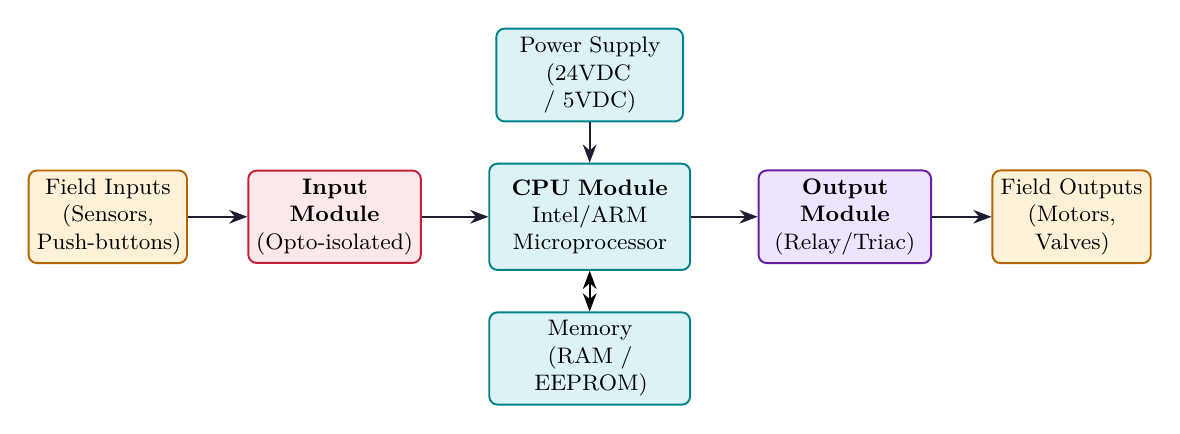
\begin{tikzpicture}[scale=0.9, transform shape]
  % Processor and Memory
  \node[block, text width=2.6cm, minimum height=1.5cm] (cpu) at (0,0) {\textbf{CPU Module}\\Intel/ARM\\Microprocessor};
  \node[block, text width=2.6cm] (mem) at (0, -2.0) {Memory\\(RAM / EEPROM)};
  
  % Input and Output Blocks
  \node[block, draw=myred, fill=hdrred, text width=2.2cm, minimum height=1.3cm] (in) at (-3.6, 0) {\textbf{Input Module}\\(Opto-isolated)};
  \node[block, draw=mypurple, fill=hdrpurple, text width=2.2cm, minimum height=1.3cm] (out) at (3.6, 0) {\textbf{Output Module}\\(Relay/Triac)};
  
  % Field Devices
  \node[block, text width=2.0cm, draw=myamber, fill=hdramber] (dev_in) at (-6.8, 0) {Field Inputs\\(Sensors, Push-buttons)};
  \node[block, text width=2.0cm, draw=myamber, fill=hdramber] (dev_out) at (6.8, 0) {Field Outputs\\(Motors, Valves)};

  % Power Supply
  \node[block, text width=2.4cm] (ps) at (0, 2.0) {Power Supply\\(24VDC / 5VDC)};

  % Internal bus paths
  \draw[Stealth-Stealth, thick] (cpu) -- (mem);
  \draw[arrow] (ps) -- (cpu);
  
  % Input/Output connections
  \draw[arrow] (dev_in) -- (in);
  \draw[arrow] (in) -- (cpu);
  \draw[arrow] (cpu) -- (out);
  \draw[arrow] (out) -- (dev_out);
\end{tikzpicture}
\end{tcolorbox}

\textbf{Core Hardware Blocks:}
\begin{enumerate}[label=\textbf{\arabic*.}, leftmargin=*]
  \item \textbf{CPU Module:} Executes the user program, updates the output image table, and diagnoses system faults.
  \item \textbf{Input Module:} Receives high-voltage field signals (e.g. $120\,$VAC, $24\,$VDC) from pushbuttons or limit switches. It uses \textbf{optical isolation} to convert the signals to low-voltage $5\,$VDC signals, protecting the CPU from electrical noise and voltage spikes.
  \item \textbf{Output Module:} Translates the CPU's logic decisions into power switching to steer load devices (solenoids, contactors, pilot lights).
    \begin{itemize}[leftmargin=*, itemsep=2pt]
      \item \textit{Relay Outputs:} Dry contacts, slow, but switch both AC/DC and handle high currents.
      \item \textit{Transistor outputs (DC only):} Fast solid-state switching, low current.
      \item \textit{Triac outputs (AC only):} Silent solid-state switching, moderate current.
    \end{itemize}
\end{enumerate}

% ===============================================================================
\section{PLC Operational Scan Cycle}
% ===============================================================================

A PLC operates by repeatedly executing a cycle of four distinct phases:

\begin{tcolorbox}[tikzbox, title={PLC Cycle Scan Flow}]
\centering
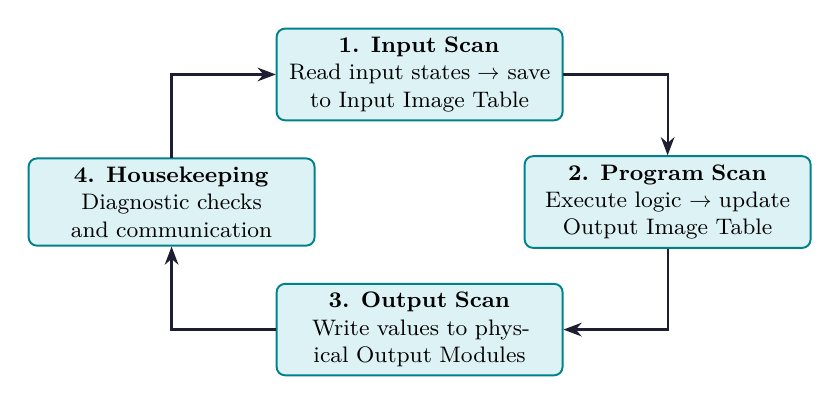
\begin{tikzpicture}[scale=0.9, transform shape]
  % Steps
  \node[block, text width=3.8cm] (step1) at (0, 1.8) {\textbf{1. Input Scan}\\Read input states $\to$ save to Input Image Table};
  \node[block, text width=3.8cm] (step2) at (3.5, 0) {\textbf{2. Program Scan}\\Execute logic $\to$ update Output Image Table};
  \node[block, text width=3.8cm] (step3) at (0, -1.8) {\textbf{3. Output Scan}\\Write values to physical Output Modules};
  \node[block, text width=3.8cm] (step4) at (-3.5, 0) {\textbf{4. Housekeeping}\\Diagnostic checks and communication};

  % Paths
  \draw[arrow] (step1) -| (step2);
  \draw[arrow] (step2) |- (step3);
  \draw[arrow] (step3) -| (step4);
  \draw[arrow] (step4) |- (step1);
\end{tikzpicture}
\end{tcolorbox}

\begin{itemize}[leftmargin=*, itemsep=2.5pt]
  \item \textbf{Scan Time:} The total time required to complete one cycle (typically $1\text{--}10\,$ms).
  \item \textbf{Watchdog Timer:} A hardware timer initialized at the start of each scan cycle. If the scan time exceeds a preset safety limit (e.g. $100\,$ms due to an infinite program loop or processor hang), the watchdog timer trips, instantly shutting down all PLC outputs for safety.
\end{itemize}


% ===============================================================================
\section{Ladder Diagram (LD) Programming}
% ===============================================================================

\subsection{1. Fundamental Instructions}
\begin{itemize}[leftmargin=*, itemsep=2.5pt]
  \item \textbf{Normally Open Contact (NO) \texttt{-[ ]-}:} Examines if a bit is ON (1). If the referenced memory bit is 1, the contact closes, allowing power flow. (Instruction: \textbf{XIC} --- Examine If Closed).
  \item \textbf{Normally Closed Contact (NC) \texttt{-[\textbackslash]-}:} Examines if a bit is OFF (0). If the referenced memory bit is 0, the contact remains closed, allowing power flow. (Instruction: \textbf{XIO} --- Examine If Open).
  \item \textbf{Output Coil \texttt{-( )}-:} Sets a referenced memory bit to 1 when power flows through the rung. (Instruction: \textbf{OTE} --- Output Energize).
  \item \textbf{Latching/Sealing:} Since industrial pushbuttons are momentary, control rungs use a parallel contact of the output coil wired around the start button to "seal in" power.
\end{itemize}

\begin{tcolorbox}[tikzbox, title={Stop-Start Motor Latching Logic (Ladder Diagram)}]
\centering
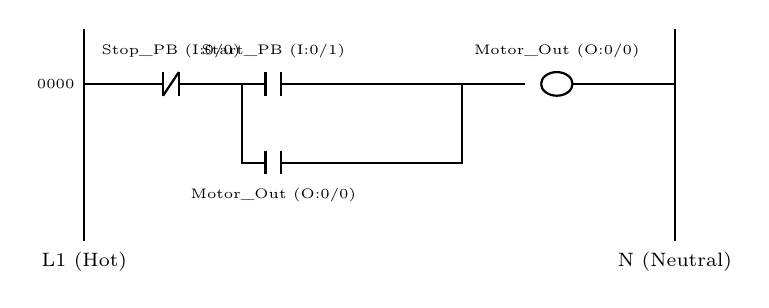
\begin{tikzpicture}[scale=1.0]
  % Rails
  \draw[thick] (0, 1.2) -- (0, -1.5) node[below, font=\scriptsize] {L1 (Hot)};
  \draw[thick] (7.5, 1.2) -- (7.5, -1.5) node[below, font=\scriptsize] {N (Neutral)};
  
  % Rung 1
  \draw[thick] (0, 0.5) -- (0.8, 0.5);
  
  % Stop Contact (NC)
  \draw[thick] (0.8, 0.5) -- (1.0, 0.5);
  \draw[thick] (1.0, 0.35) -- (1.0, 0.65);
  \draw[thick] (1.0, 0.35) -- (1.2, 0.65);
  \draw[thick] (1.2, 0.35) -- (1.2, 0.65);
  \draw[thick] (1.2, 0.5) -- (2.0, 0.5);
  \node[above, font=\tiny] at (1.1, 0.7) {Stop\_PB (I:0/0)};

  % Start Contact (NO)
  \draw[thick] (2.0, 0.5) -- (2.3, 0.5);
  \draw[thick] (2.3, 0.35) -- (2.3, 0.65);
  \draw[thick] (2.5, 0.35) -- (2.5, 0.65);
  \draw[thick] (2.5, 0.5) -- (4.8, 0.5);
  \node[above, font=\tiny] at (2.4, 0.7) {Start\_PB (I:0/1)};
  
  % Seal-in Contact (NO) in parallel
  \draw[thick] (2.0, 0.5) -- (2.0, -0.5) -- (2.3, -0.5);
  \draw[thick] (2.3, -0.65) -- (2.3, -0.35);
  \draw[thick] (2.5, -0.65) -- (2.5, -0.35);
  \draw[thick] (2.5, -0.5) -- (4.8, -0.5) -- (4.8, 0.5);
  \node[below, font=\tiny] at (2.4, -0.7) {Motor\_Out (O:0/0)};
  
  % Output Coil
  \draw[thick] (4.8, 0.5) -- (5.6, 0.5);
  \draw[thick] (5.8, 0.5) arc (0:180:-0.2 and 0.15);
  \draw[thick] (5.8, 0.5) arc (0:180:-0.2 and -0.15);
  \draw[thick] (6.2, 0.5) -- (7.5, 0.5);
  \node[above, font=\tiny] at (6.0, 0.7) {Motor\_Out (O:0/0)};
  
  % Bounding box rung labels
  \node[left, font=\tiny] at (0, 0.5) {0000};
\end{tikzpicture}
\end{tcolorbox}

\subsection{2. Timers and Counters}
\begin{itemize}[leftmargin=*, itemsep=2.5pt]
  \item \textbf{Timer On-Delay (TON):} When the rung becomes true, the timer begins accumulating time. Once the Accumulated Value (ACC) equals the Preset Value (PRE), the \textbf{Done Bit (DN)} is set to 1. If the rung goes false, ACC resets to 0.
  \item \textbf{Timer Off-Delay (TOF):} The DN bit is set to 1 immediately when the rung becomes true. When the rung goes false, the timer starts counting. Once ACC equals PRE, the DN bit resets to 0.
  \item \textbf{Retentive Timer (RTO):} Retains its ACC value even if the rung goes false. A separate \textbf{Reset (RES)} instruction is required to clear ACC back to 0.
  \item \textbf{Counters (CTU/CTD):} Count up (CTU) or down (CTD) on each false-to-true rung transition of their input. The DN bit is set to 1 when ACC matches PRE.
\end{itemize}

% ===============================================================================
\section{Industrial PLC Application Examples}
% ===============================================================================

\subsection{Automatic Tank/Bottle Filling Logic}
\begin{itemize}[leftmargin=*, itemsep=2.5pt]
  \item \textbf{Process Description:} A bottle arrives on a conveyor belt. When the proximity sensor detects the bottle, the conveyor stops, and a solenoid valve opens to fill the bottle. A level sensor detects when the bottle is full, closing the valve and restarting the conveyor.
  \item \textbf{Ladder Logic Allocation:}
    \begin{itemize}[leftmargin=*, itemsep=2pt]
      \item Inputs: \texttt{Start\_PB} (I:0/0), \texttt{Stop\_PB} (I:0/1), \texttt{Prox\_Sensor} (I:0/2), \texttt{Level\_Sensor} (I:0/3).
      \item Outputs: \texttt{Conveyor\_Motor} (O:0/0), \texttt{Fill\_Valve} (O:0/1).
    \end{itemize}
  \item \textbf{Rungs Description:}
    \begin{itemize}[leftmargin=*, itemsep=2pt]
      \item \textbf{Rung 1 (Conveyor Run):} Run the conveyor motor if the system is started, and stop it if the \texttt{Prox\_Sensor} detects a bottle OR the \texttt{Stop\_PB} is pressed.
      \item \textbf{Rung 2 (Fill Valve Run):} Open the fill valve if a bottle is present (\texttt{Prox\_Sensor} is true) and the bottle is not yet full (\texttt{Level\_Sensor} is false).
    \end{itemize}
\end{itemize}

\newpage

% ===============================================================================
% QUICK REVISION PAGE
% ===============================================================================
\begin{center}
  {\large\bfseries\color{myred} Quick Revision --- Module 4}\\[3pt]
  {\small\color{mydark} PLC Systems $|$ PE-EC802B}
\end{center}
\noindent{\color{myred}\rule{\linewidth}{1.2pt}}
\vspace{4pt}

\begin{tcolorbox}[defbox, title={\textbf{One-Line Definitions}}]
\begin{itemize}[leftmargin=*, itemsep=2pt, topsep=0pt]
  \item \textbf{PLC:} A solid-state industrial control computer designed to execute logic programs recursively in real-time.
  \item \textbf{Scan Cycle:} The recursive loop of reading physical inputs, executing code, and updating physical outputs.
  \item \textbf{Watchdog Timer (WDT):} A hardware safety timer that shuts down the PLC if the scan time exceeds a set limit.
  \item \textbf{Optical Isolation:} Using LED-phototransistor pairs to separate high-voltage field wiring from CPU logic circuit.
  \item \textbf{XIC (Examine If Closed):} Contact instruction that is logically true when the referenced memory bit is 1.
  \item \textbf{XIO (Examine If Open):} Contact instruction that is logically true when the referenced memory bit is 0.
  \item \textbf{Seal-in Contact:} A parallel contact of an output coil used to maintain power flow after a momentary button is released.
\end{itemize}
\tcbset{breakable}
\end{tcolorbox}

\begin{tcolorbox}[tikzbox, title={\textbf{Output Module \& Timer Comparisons}}]
\centering
\par\noindent
\renewcommand{\arraystretch}{1.3}
\begin{tabularx}{\linewidth}{|B{3.0cm}|Y|Y|Y|}
\hline
\textbf{Property} & \textbf{Relay Output} & \textbf{Transistor Output} & \textbf{Triac Output} \\ \hline
\textbf{Load Type} & Both AC and DC & DC only & AC only \\ \hline
\textbf{Switch Speed} & Slow ($\sim 10\,$ms) & Very Fast ($< 1\,\mu$s) & Fast (crosses zero, $\sim 8\,$ms) \\ \hline
\textbf{Wear / Lifetime} & Limited (mechanical wear) & Infinite (solid-state) & Infinite (solid-state) \\ \hline
\textbf{Isolation} & Inherently isolated & Requires optocoupler & Requires optocoupler \\ \hline
\end{tabularx}

\vspace{0.3cm}
\begin{tabularx}{\linewidth}{|B{3.0cm}|Y|Y|}
\hline
\textbf{Property} & \textbf{Timer On-Delay (TON)} & \textbf{Timer Off-Delay (TOF)} \\ \hline
\textbf{Enable condition} & Rung must be TRUE to count time & Rung must transition TRUE $\to$ FALSE to count \\ \hline
\textbf{DN Bit Action} & Set to 1 once Preset time is reached & Set to 1 instantly; resets once Preset time is reached \\ \hline
\textbf{Loss of Rung} & ACC value resets instantly to 0 & ACC value resets instantly to 0 \\ \hline
\end{tabularx}
\end{tcolorbox}

\begin{tcolorbox}[exambox, title={\textbf{Frequently Asked / Viva Questions}}]
\begin{enumerate}[leftmargin=*, itemsep=4pt]
  \item \Q{Describe the sequence of operations in a single PLC scan cycle.}
    A scan cycle consists of four sequential steps: (1) \textbf{Input Scan:} reads physical input module terminals and copies states into the Input Image Table. (2) \textbf{Program Scan:} runs the user ladder logic code sequentially, updating the Output Image Table. (3) \textbf{Output Scan:} copies Output Image Table states to the physical output module terminals. (4) \textbf{Housekeeping:} runs communication and processor diagnostics.
  \item \Q{Why is optical isolation used in PLC input modules?}
    Field input devices (limit switches, sensors) operate on high voltages ($24\,$VDC, $120\,$VAC) and are exposed to industrial surges and electromagnetic noise. Optical isolation separates the field wiring from the $5\,$VDC CPU logic using LED-photodiode pairs, preventing high-voltage transients from destroying the processor.
  \item \Q{Compare Relay, Transistor, and Triac output modules in PLCs.}
    Relay output modules are mechanical switches that handle high currents and switch both AC and DC, but are slow and wear out. Transistor output modules are solid-state switches that only handle DC, switch extremely fast, and have an infinite life. Triac output modules are solid-state switches designed for AC only.
  \item \Q{What is the function of the Watchdog Timer (WDT) in a PLC?}
    The WDT is a safety timer that monitors the scan cycle. If the program gets stuck in an infinite loop or the CPU freezes, the scan cycle fails to complete. When the WDT exceeds its preset threshold, it trips, putting the PLC in a "fault" state and turning off all outputs to prevent runaway machine actions.
  \item \Q{State the difference between TON, TOF, and RTO timers.}
    TON (Timer On-Delay) starts counting when its rung becomes true and sets its DN bit when ACC reaches PRE. TOF (Timer Off-Delay) turns on its DN bit immediately when the rung goes true, starts counting when the rung goes false, and resets DN when ACC reaches PRE. RTO (Retentive Timer) behaves like TON but does not reset its ACC value when the rung goes false; it requires an explicit RES instruction.
  \item \Q{How is a seal-in circuit implemented in Ladder Logic, and why is it necessary?}
    It is implemented by wiring a normally open contact of the output coil in parallel with the momentary Start pushbutton contact. When the Start button is pressed, the coil energizes and closes the parallel contact. When the Start button is released, current continues to flow through the parallel contact (sealing it in) until a series Stop pushbutton opens the rung.
\end{enumerate}
\end{tcolorbox}

\end{document}
